% Lecture 1: continuum hypothesis - problem scale >> fluid element >> molecular scale
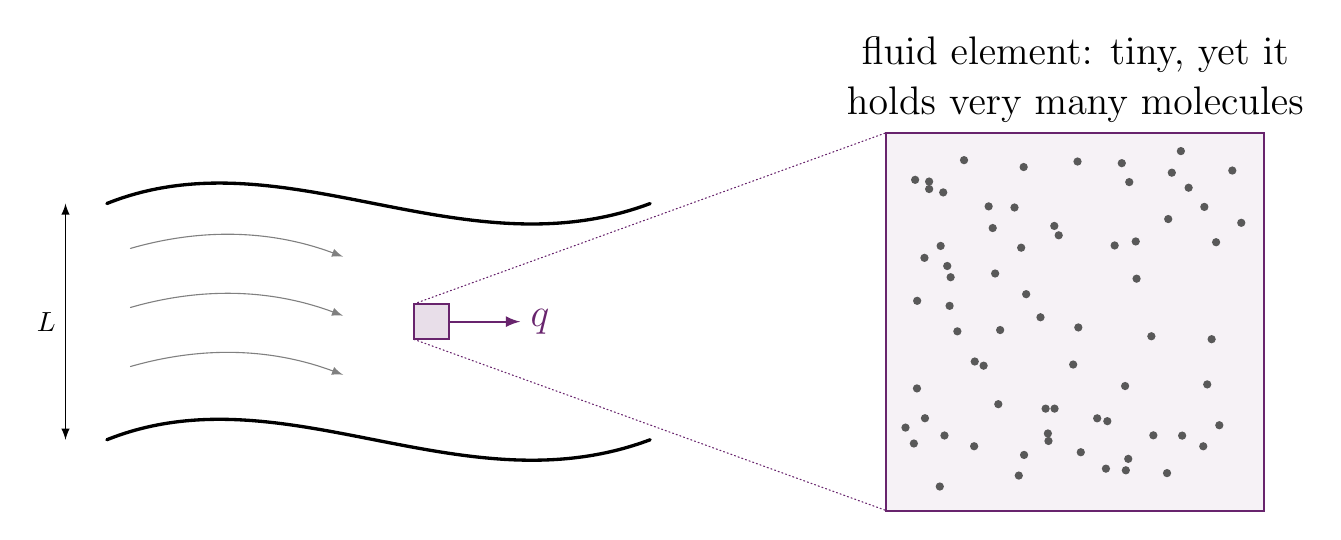
\begin{tikzpicture}[scale=1.5, >=latex, line cap=round]
  \definecolor{dpurple}{HTML}{68246D}
  % channel (problem scale)
  \draw[very thick] (0,2.0) .. controls (1.5,2.6) and (3,1.4) .. (4.6,2.0);
  \draw[very thick] (0,0) .. controls (1.5,0.6) and (3,-0.6) .. (4.6,0);
  \foreach \y in {0.5,1.0,1.5} \draw[->, gray] (0.2,\y+0.12) .. controls (1,\y+0.35) and (1.6,\y+0.2) .. (2.0,\y+0.05);
  \draw[<->] (-0.35,0) -- (-0.35,2.0) node[midway, left] {$L$};
  % fluid element
  \draw[thick, dpurple, fill=dpurple!15] (2.6,0.85) rectangle (2.9,1.15);
  \draw[->, thick, dpurple] (2.9,1.0) -- (3.5,1.0) node[right, font=\Large] {$\vect{q}$};
  % zoom
  \draw[dpurple, densely dotted] (2.6,1.15) -- (6.6,2.6);
  \draw[dpurple, densely dotted] (2.6,0.85) -- (6.6,-0.6);
  \draw[thick, dpurple, fill=dpurple!6] (6.6,-0.6) rectangle (9.8,2.6);
  \pgfmathsetseed{7}
  \foreach \i in {1,...,70} {
    \pgfmathsetmacro{\px}{6.75+2.9*rnd}\pgfmathsetmacro{\py}{-0.45+2.9*rnd}
    \fill[black!65] (\px,\py) circle (0.035);
  }
  \node[font=\Large, align=center] at (8.2,3.05) {fluid element: tiny, yet it\\ holds very many molecules};
\end{tikzpicture}
